% LaTeX file for resume
% This file uses the resume document class (res.cls)
\documentclass[12pt]{article}
\usepackage[utf8]{inputenc}
\usepackage{amsmath}
\usepackage{amsfonts}
\usepackage{amssymb}


\usepackage[usenames, dvipsnames]{xcolor}
\usepackage[colorlinks = true,urlcolor = BrickRed,pdfnewwindow=true]{hyperref}

% \usepackage{graphicx}
% \graphicspath{‎{}}

\usepackage{datetime}
\newdateformat{monthyeardate}{%
  \monthname[\THEMONTH], \THEYEAR}


\usepackage[framemethod=tikz]{mdframed}
\newmdenv[innerlinewidth=0.8pt, roundcorner=4pt,linecolor=RoyalBlue,innerleftmargin=6pt,
innerrightmargin=6pt,innertopmargin=6pt,innerbottommargin=6pt]{mybox}
\usepackage{wrapfig}

\usepackage{titlesec}
\titleformat{\section}[block]{\large}{\textbf{\thesection}}{1em}{ \bfseries}
\titleformat{\subsection}[block]{\hspace{0.6em}}{\textbf{\thesubsection}}{1em}{\bfseries}

\definecolor{blanc}{rgb}{1,1,1}
\usepackage{etaremune}

\usepackage{fancyhdr}  % use this package to get a 2 line header
\renewcommand{\headrulewidth}{0pt} % suppress line drawn by default by fancyhdr

\setlength{\headsep}{20pt}  % space between header and text
\setlength{\footskip}{29pt}
\pagestyle{fancy}     % set pagestyle for document
\rhead{} % put text in header (right side)

\rhead{\textcolor{Gray}{ \thepage/10}}

\chead{\textcolor{Gray}{}} % put text in header (right side)
\cfoot{}

\lfoot{\textcolor{Gray}{CV last update: \monthyeardate\today}}
\rfoot{\href{http://johanmazoyer.com}{johanmazoyer.com}}

\setlength{\parindent}{0pt}

\setlength{\headwidth}{6.5in} % taille de l'entete
\usepackage[total={6.5in,9in},left=1in,top=1in,headheight=110pt]{geometry} %%%%% 8.5in x 11in




\begin{document}
\lhead[]{}
% \textcolor{blanc}{.}
% \vspace{-1.cm}

\begin{huge}
\noindent\textbf{Johan MAZOYER}
\end{huge}\\

%\vspace{-0.3cm}
%\textit{French citizen, born on December $14^{th}$ 1986, Paris, France.}

\textbf{Research Interests: Optical Instrumentation, Direct Imaging \& Coronagraphy,
Observation \& Characterization of Extrasolar Systems, Debris Disks}\\


%%%%%%%%%%%%%%%%%%%%%%%%%%%%%%%%%%%%%%%%%%%%%%%%%%%%%%%%%%%%%%%%%%%%%%%%%%%%%%%%%%%%%%%%%%%%%%%%%%%%%%%%%%%%%%%%%%%%%%%%
%%%%%% SECTION RESEARCH EXPERIENCE
%%%%%%%%%%%%%%%%%%%%%%%%%%%%%%%%%%%%%%%%%%%%%%%%%%%%%%%%%%%%%%%%%%%%%%%%%%%%%%%%%%%%%%%%%%%%%%%%%%%%%%%%%%%%%%%%%%%%%%%%
\vspace{-1cm}
\textcolor{RoyalBlue}{\section{\large RESEARCH POSITIONS}
\vspace{-0.35cm}\hrule}
\vspace{0.4cm}

\textbf{Chargé de recherche CNRS} --
\href{http://www.obspm.fr/?lang=en}{\textbf{LESIA/Paris Observatory}}
\hfill     	 { \bf starting 2020}\\


\textbf{Carl Sagan Postdoctoral Fellow} --
\href{https://www.jpl.nasa.gov/}{\textbf{Jet Propulsion Laboratory}}
\hfill      { \bf 2018 - 2019}\\


\textbf{Postdoctoral Researcher} --
\href{http://physics-astronomy.jhu.edu/}{\textbf{Johns Hopkins University}}
\hfill   	 { \bf 2016 - 2018}\\


\textbf{Postdoctoral Researcher} --
{\href{http://www.stsci.edu}{\textbf{Space Telescope Science Institute}}}
\hfill        { \bf 2014 - 2016}\\

\textbf{Graduate Student} --
\href{http://www.obspm.fr/?lang=en}{\textbf{LESIA/Paris Observatory}}
\hfill        { \bf 2011 - 2014}\\


% \vspace{-0.1cm}
% {\small \textbf{Visiting Research Student} -- \href{http://www.lanl.gov/}{\textbf{Los Alamos National Laboratory} } \hfill    	Los Alamos, NM\\
% MSL/ChemCam Collaboration (Roger Wiens) \hfill  		 \textbf{Summer 2011}\\

% \vspace{-0.1cm}
% \textbf{Visiting Research Student} -- \href{http://www.irap.omp.eu/en}{\textbf{IRAP}} \hfill    	Toulouse, Fr\\
% MSL/ChemCam Collaboration (Olivier Gasnault \& Sylvestre Maurice) \hfill		  \textbf{Spring 2011}}\\

%\vspace{-0.35cm}
%{\small \textbf{CNES} (French space agency) \hfill    	Toulouse, France\\
%\textit{Master student} ; Pleiades satellites \hfill  		 {\bf March -- July 2010}}\\
%
%\vspace{-0.35cm}
%{\small\textbf{Le Relais} (French NGO) \hfill    		  Koudougou, Burkina Faso\\
%Humanitarian work\hfill  		  {\bf July -- Sept. 2009}}	\\

%%%%%%%%%%%%%%%%%%%%%%%%%%%%%%%%%%%%%%%%%%%%%%%%%%%%%%%%%%%%%%%%%%%%%%%%%%%%%%%%%%%%%%%%%%%%%%%%%%%%%%%%%%%%%%%%%%%%%%%%
%%%%%% SECTION EDUCATION
%%%%%%%%%%%%%%%%%%%%%%%%%%%%%%%%%%%%%%%%%%%%%%%%%%%%%%%%%%%%%%%%%%%%%%%%%%%%%%%%%%%%%%%%%%%%%%%%%%%%%%%%%%%%%%%%%%%%%%%%

\vspace{-0.25cm}
\textcolor{RoyalBlue}{\section{\large EDUCATION}
\vspace{-0.35cm}\hrule}
\vspace{0.4cm}

PhD -- \textbf{Astronomy \& Astrophysics} --
\href{https://www.univ-paris-diderot.fr/}{\textbf{Universit\'e Paris Diderot}}
\hfill  { \bf 2014}\\
{\small
\textcolor{blanc}{.}\hspace{0.8cm}
{\it Thesis Advisors}: P. Baudoz \& G. Rousset \\
\textcolor{blanc}{.}\hspace{0.8cm}
{\it Thesis}: High-Contrast Direct Imaging Of Exoplanets And Circumstellar Disks}\\

% \vspace{-0.1cm}
Master --  \textbf{Astronomy \& Astrophysics}  --
\href{http://ezomp2.omp.obs-mip.fr/asep/index.php/eng}{\textbf{Université Toulouse Paul Sabatier} }
\hfill  { \bf 2011} \\
{\small
\textcolor{blanc}{.}\hspace{0.8cm}
{\it Master Thesis Advisors}: O. Gasnault (IRAP) \& R. Wiens (LANL)\\
\textcolor{blanc}{.}\hspace{0.8cm}
{\it Thesis}: Influence of Mars atmosphere on the ChemCam abundance detection limits}\\

% \vspace{-0.1cm}
Master -- \textbf{Space Engineering} -- \href{https://www.isae-supaero.fr/en/}{\textbf{\textbf{ISAE Supaero} }} \hfill  { \bf 2011} \\

% \vspace{-0.1cm}
Bachelor -- \textbf{Computer Science} -- \href{http://www.polytechnique.edu/en/}{\textbf{\textbf{Ecole polytechnique} }}  \hfill    { \bf 2010 }\\





%%%%%%%%%%%%%%%%%%%%%%%%%%%%%%%%%%%%%%%%%%%%%%%%%%%%%%%%%%%%%%%%%%%%%%%%%%%%%%%%%%%%%%%%%%%%%%%%%%%%%%%%%%%%%%%%%%%%%%%%
%%%%%% SECTION AWARDS
%%%%%%%%%%%%%%%%%%%%%%%%%%%%%%%%%%%%%%%%%%%%%%%%%%%%%%%%%%%%%%%%%%%%%%%%%%%%%%%%%%%%%%%%%%%%%%%%%%%%%%%%%%%%%%%%%%%%%%%%

\vspace{-0.25cm}
\textcolor{RoyalBlue}{\section{\large GRANTS \& AWARDS}
\vspace{-0.45cm}\hrule}
\vspace{0.4cm}
\textbf{Carl Sagan Fellowship} (\href{http://www.stsci.edu/stsci-research/fellowships/nasa-hubble-fellowship-program}{NASA Hubble Fellowship Program}) \hfill   \textbf{2018}\\ %- \$300K/3 yrs

% \vspace{-0.1cm}
Cover of \textbf{Astronomy \& Astrophysics} Journal (\href{https://www.aanda.org/articles/aa/abs/2014/04/contents/contents.html}{Volume 564}) \hfill  \textbf{2014}\\

% \vspace{-0.1cm}
\textbf{Outstanding Presentation Award} (CNES fellow symposium JC$^2$) \hfill   \textbf{2013}\\

% \vspace{-0.1cm}
\textbf{CNES Doctoral Research Fellowship} (\href{https://cnes.fr/en/web/CNES-en/7430-research-grants.php}{French space agency})  \hfill   \textbf{2011}\\ %- \$66K/3 yrs

% \vspace{-0.1cm}
\textbf{Ecole Polytechnique Scholarship}   \hfill   \textbf{2007}\\

%%%%%%%%%%%%%%%%%%%%%%%%%%%%%%%%%%%%%%%%%%%%%%%%%%%%%%%%%%%%%%%%%%%%%%%%%%%%%%%%%%%%%%%%%%%%%%%%%%%%%%%%%%%%%%%%%%%%%%%%
%%%%%% SECTION VULGARISATION
%%%%%%%%%%%%%%%%%%%%%%%%%%%%%%%%%%%%%%%%%%%%%%%%%%%%%%%%%%%%%%%%%%%%%%%%%%%%%%%%%%%%%%%%%%%%%%%%%%%%%%%%%%%%%%%%%%%%%%%%

\newpage
\textcolor{White}{.}
%\lhead{\textcolor{Gray}{J. MAZOYER}}
\vspace{-1.5cm}
\textcolor{RoyalBlue}{\section{\large OUTREACH}
\vspace{-0.35cm}\hrule}
\vspace{0.5cm}
\begin{wrapfigure}{l}{0.26\textwidth}
\vspace{-0.95cm}
\begin{mybox}
    
\includegraphics[width=1.\textwidth]{figures_CV/PodcastScience.png}
 \end{mybox}
\vspace{-1.1cm}
\end{wrapfigure}
\textbf{Podcast Science}: I am running \href{http://www.podcastscience.fm}
{\textbf{PodcastScience.fm}}, a \textbf{general science program}, airing every
Wednesdays, in french. This podcast is listened by 10'000 to 20'000
listeners. Podcast Science received the Golden blog award for
best scientific blog in 2012.

\vspace{0.5cm}
\textbf{Kidi'Science}: Contributor for this children science blog.\\

\textbf{Public talks}: CERN \& Palais de la découverte (Paris)\\

\vspace{-0.3cm}
\textcolor{RoyalBlue}{\section{\large PROFESSIONAL ACTIVITIES \& SERVICE}
\vspace{-0.35cm}\hrule}
\vspace{0.6cm}

\parbox{0.55\linewidth}{
\textbf{Conference and Workshop Organizer:}
\begin{itemize}
 \item \small Organizer and SOC: \textbf{National Capital Area Disks} workshop (Baltimore, MD, Oct. 2018) - \href{https://sites.google.com/view/ncad7-at-jhu/ncad7}{\underline{\textbf{website}}}
 \item \small Organizer and SOC: \textbf{Optimal Optical Coronagraphs} workshop (Leiden, NL, Sep. 2017) - \href{https://www.lorentzcenter.nl/lc/web/2017/924/info.php3?wsid=924&venue=Snellius}{\underline{\textbf{website}}}
 \item \small SOC: \textbf{High Contrast Imaging from Space} (Baltimore, MD, Nov. 2016) - \href{http://www.cvent.com/events/high-contrast-imaging-in-space-workshop/event-summary-eb3bb6bd54a342c5a15678daa49be683.aspx}{\underline{\textbf{website}}}
 \item \small LOC: \textbf{La très haute dynamique} workshop (Paris, FR, 2012)
\end{itemize}
\vspace{0.4cm}
\textbf{Other Services:}
\begin{itemize}
	% \item \small Member of the \textbf{WFIRST Science Investigation Team} (SIT) for disk science since 2017.
    \item \small \textbf{Hubble \textit{Telescope Allocation Committee}} panel support (2016).
\end{itemize}}
\hspace{0.2cm}
\parbox{0.43\linewidth}{
\vspace{-0.8cm}
\begin{mybox}
    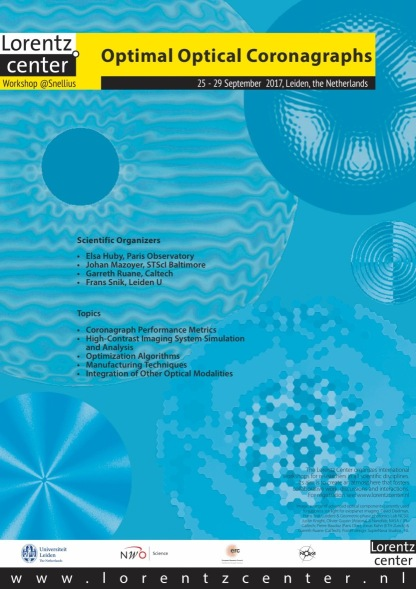
\includegraphics[width=1.\textwidth]{figures_CV/ooc_poster2_sm.jpg}
 \end{mybox}
}



\begin{itemize}
    \item \small NASA Exoplanet Exploration Program Analysis Group (ExoPAG) member of the \textbf{Study Analysis Groups (SAGs) \#19} (Theory and Rigorous Contrast Metrics) since 2016 (see Jensen-Clem et al. 2018).
    \item \small Organization of the \textbf{``Exoplanet Star and Planet Formation" (ESPF) seminar} at STScI each week (2016-2018) - \href{https://sites.google.com/site/starandplanetformationseries/}{\underline{\textbf{website}}}
    \item \small Development of the \textbf{Paris THD optical testbed website} in August 2014.
    \item \small \textbf{Referee} for publications in the \textit{AJ}, \textit{A}\&\textit{A}, \textit{MNRAS}, \textit{PASP} and \textit{JATIS}.
\end{itemize}

%\vspace{-1.cm}
%\textcolor{RoyalBlue}{\section{\large MAIN OBSERVATION CAMPAIGNS}
%\vspace{-0.35cm}\hrule}
%\vspace{0.22cm}
%
%\textbf{Palomar Observatory (200 inch telescope)}
%
%\begin{itemize} \itemsep -1pt % reduce space between items
%	    \item \small Mai 2015, 3 nights -- First on-sky test of the Self-Coherent Camera
%\end{itemize}
%
%\textbf{Gemini South/GPI}
%\vspace{-0.2cm}
%\begin{itemize} \itemsep -1pt % reduce space between items
%	    \item \small December 2015, 1 week -- Remote observing and data reduction
%		\item \small March 2016, 1 week --  Remote observing and data reduction
% 	\item \small October 2016, 1 week --  On-site observing and data reduction\\
%Since the end of 2016, all south Gemini observations are carried out remotely.
% 	\item \small December 2016, 4 nights --  Assistance and data reduction
% 	\item \small December 2017, 3 nights --  Assistance and data reduction
% 	\item \small January 2018, 4 nights --  Remote observing and data reduction
%\end{itemize}

%%%%%%%%%%%%%%%%%%%%%%%%%%%%%%%%%%%%%%%%%%%%%%%%%%%%%%%%%%%%%%%%%%%%%%%%%%%%%%%%%%%%%%%%%%%%%%%%%%%%%%%%%%%%%%%%%%%%%%%%
%%%%%% Demandes de temps
%%%%%%%%%%%%%%%%%%%%%%%%%%%%%%%%%%%%%%%%%%%%%%%%%%%%%%%%%%%%%%%%%%%%%%%%%%%%%%%%%%%%%%%%%%%%%%%%%%%%%%%%%%%%%%%%%%%%%%%%

%\vspace{-0.8cm}
%\textcolor{RoyalBlue}{\section{\large OBSERVATION PROPOSALS}
%\vspace{-0.35cm}\hrule}
%\vspace{0.4cm}
%
%\textbf{GEMINI/GPI}\\
%\vspace{-0.4cm}
%\begin{itemize} \itemsep -3pt % reduce space between items
%    \item \small GS-2015B-LP-6 ``Characterizing Dusty Debris in Exoplanetary Systems'' (PI: Christine Chen)\\
%\end{itemize}
%
%\vspace{-0.4cm}
%\textbf{VLT/SPHERE}
%\vspace{-0.2cm}
%\begin{itemize} \itemsep -3pt % reduce space between items
%    \item \small P 098.C-0686 ``Resolving multiple belts and sub-structures in inner regions of highly inclined debris disk" (PI: Anthony Boccaletti)
%    \item \small P 096.C-0640 ``Exploring the inner cavities of two very inclined debris disks'' (PI: Anthony Boccaletti)
%    \item \small P 095.C-0381 ``Investigating the inner part of a transitional disk"'' (PI: Anthony Boccaletti)
%\end{itemize}
%
%\textbf{JWST / MIRI, NIRCam, NIRSPEC \& NIRISS}
%\vspace{-0.2cm}
%\begin{itemize} \itemsep -3pt % reduce space between items
%    \item \small Programme Early realease Science (ERS) ``High Contrast Imaging of Exoplanets and Exoplanetary Systems with JWST" (PI : Sasha Hinkley)
%\end{itemize}

%%%%%%%%%%%%%%%%%%%%%%%%%%%%%%%%%%%%%%%%%%%%%%%%%%%%%%%%%%%%%%%%%%%%%%%%%%%%%%%%%%%%%%%%%%%%%%%%%%%%%%%%%%%%%%%%%%%%%%%%
%%%%%% SECTION RESPONSABILITE
%%%%%%%%%%%%%%%%%%%%%%%%%%%%%%%%%%%%%%%%%%%%%%%%%%%%%%%%%%%%%%%%%%%%%%%%%%%%%%%%%%%%%%%%%%%%%%%%%%%%%%%%%%%%%%%%%%%%%%%%

\newpage
\vspace{-0.5cm}
\textcolor{RoyalBlue}{\section{\large TEACHING \& MENTORING}
\vspace{-0.35cm}\hrule}
\vspace{0.4cm}

\textbf{PhD supervising:}\\
\begin{itemize}
    \item \small  \textbf{Lucie Leboulleux}, in co-direction between STScI \& ONERA, France (Leboulleux, N'Diaye, Mazoyer  et al. 2017 SPIE ; Leboulleux et al. 2018 ;  Leboulleux et al. 2018 SPIE).
    \item \textbf{Kevin Fogarty}, PhD at JHU and 1 year postdoc at STScI (Fogarty, Pueyo, Mazoyer et al, 2018 AJ ; Fogarty, Mazoyer et al, 2018 SPIE ; Fogarty, Pueyo, Mazoyer et al, 2017 SPIE). Now Caltech Prize Postdoctoral Fellowship in Experimental Physics or Astrophysics.
    % \item \textbf{Sylvain Egron}, in co-direction between STScI \& ONERA, France (Egron et al. 2017 SPIE)\\
\end{itemize}

\textbf{Teaching assistant:}\\
\vspace{-0.2cm}

\textbf{Universit\'e Paris Diderot -- Paris 7} \hspace{1.85cm} {\small Electronics} \hfill \textbf{2013 - 2014}\\
\textbf{Universit\'e Paris Descartes -- Paris 5} \hspace{1.5cm} {\small Fluid dynamics} \hfill \textbf{2011 - 2012}\\

\textbf{La Main à la Pâte:} \hfill \textbf{2007 - 2008}
\begin{itemize}
    \item {\small I taught science during 8 months (30h/week) in primary schools in underprivileged neighborhoods (Perpignan, France). \href{https://www.fondation-lamap.org/en/international}{\textbf{La Main à la pâte}} was  founded by Nobel Prize winner G. Charpak, astronomer P. Léna and physicist Y. Quéré, of the French Academy of Sciences, to improve the quality of science and technology teaching in primary and middle school.}
\end{itemize}




%\vspace{-0.5cm}
%\textcolor{RoyalBlue}{\section{\large  SPORT}
%\vspace{-0.35cm}\hrule}
%\vspace{0.4cm}
%\textbf{Fencing} (15 years of practice) \& \textbf{Running} (trails, half-marathons, marathon)\\

\newpage

\textcolor{White}{.}
\vspace{-1.cm}
\begin{center}
\begin{Large}
\textbf{PUBLICATIONS \& PRESENTATIONS}\\
\end{Large}
\setcounter{section}{0}
\end{center}
\vspace{-0.8cm}
\textcolor{RoyalBlue}{\section{\large REFEREED PUBLICATIONS  IN FIRST AUTHOR}
\vspace{-0.35cm}\hrule}
\vspace{0.6cm}

\begin{etaremune}
\item \textbf{Mazoyer, J.}, Pueyo, L., N’Diaye, M., Fogarty, K., Zimmerman, N., Soummer, R., Shaklan, S. and Norman, C., “Active Correction of Aperture Discontinuities-Optimized Stroke Minimization. II. Optimization for Future Missions,” The Astronomical Journal 155, 8, 19 pages (\textbf{2018}).\\
Link: \textcolor{BrickRed}{\underline{\url{http://adsabs.harvard.edu/abs/2018AJ....155....8M}}}
\item \textbf{Mazoyer, J.}, Pueyo, L., N’Diaye, M., Fogarty, K., Zimmerman, N., Leboulleux, L., St. Laurent, K. E., Soummer, R., Shaklan, S. and Norman, C., “Active Correction of Aperture Discontinuities-Optimized Stroke Minimization. I. A New Adaptive Interaction Matrix Algorithm,” The Astronomical Journal 155, 7, 13 pages (\textbf{2018}).\\
Link: \textcolor{BrickRed}{\underline{\url{http://adsabs.harvard.edu/abs/2018AJ....155....7M}}}
\item \textbf{Mazoyer, J.}, Boccaletti, A., Choquet, É., Perrin, M. D., Pueyo, L., Augereau, J.-C., Lagrange, A.-M., Debes, J. and Wolff, S. G., “A Symmetric Inner Cavity in the HD 141569A Circumstellar Disk,” The Astrophysical Journal 818(2), 150, 8 pages (\textbf{2016}).\\
Link: \textcolor{BrickRed}{\underline{\url{http://adsabs.harvard.edu/abs/2016ApJ...818..150M}}}
\item \textbf{Mazoyer, J.}, Pueyo, L., Norman, C., N’Diaye, M., van der Marel, R. P. and Soummer, R., “Active compensation of aperture discontinuities for WFIRST-AFTA: analytical and numerical comparison of propagation methods and preliminary results with a WFIRST-AFTA-like pupil,” Journal of Astronomical Telescopes, Instruments, and Systems 2, 011008, 8 pp (\textbf{2016}).\\
Link: \textcolor{BrickRed}{\underline{\url{http://adsabs.harvard.edu/abs/2016JATIS...2a1008M}}}
\item \textbf{Mazoyer, J.}, Boccaletti, A., Augereau, J.-C., Lagrange, A.-M., Galicher, R. and Baudoz, P., “Is the HD 15115 inner disk really asymmetrical?,” Astronomy and Astrophysics 569, A29, 9 pages (\textbf{2014}).\\
Link: \textcolor{BrickRed}{\underline{\url{http://adsabs.harvard.edu/abs/2014A\%26A...569A..29M}}}
\item \textbf{Mazoyer, J.}, Baudoz, P., Galicher, R. and Rousset, G., “High-contrast imaging in polychromatic light with the self-coherent camera,” Astronomy and Astrophysics 564, L1, 4 pages (\textbf{2014}). \\ \textcolor{RoyalBlue}{\textbf{Made the front cover of Astronomy \& Astrophysics in April 2014}}\\
Link: \textcolor{BrickRed}{\underline{\url{http://adsabs.harvard.edu/abs/2014A\%26A...564L...1M}}}

\item \textbf{Mazoyer, J.}, Baudoz, P., Galicher, R., Mas, M. and Rousset, G., “Estimation and correction of wavefront aberrations using the self-coherent camera: laboratory results,” Astronomy and Astrophysics 557, 9, 13 pages (\textbf{2013}).\\
Link: \textcolor{BrickRed}{\underline{\url{http://adsabs.harvard.edu/abs/2013A\%26A...557A...9M}}}
\end{etaremune}

\vspace{-0.8cm}
\textcolor{RoyalBlue}{\section{\large OTHER REFEREED PUBLICATIONS}
\vspace{-0.35cm}\hrule}
\vspace{0.3cm}

\begin{etaremune}
\item Bhowmik, T., Boccaletti, A., Thébault, P., Kral, Q., \textbf{Mazoyer, J.} et al.,
"Spatially resolved spectroscopy of the debris disk HD 32297: Further evidence of small dust grains"
accepted in Astronomy and Astrophysics (\textbf{2019}).\\
Link: \textcolor{BrickRed}{\underline{\url{https://ui.adsabs.harvard.edu/abs/2019arXiv190808511B/abstract}}}
\item Ren, B.; Choquet, É.; Perrin, M. D.; Duchêne, G. et al., "An Exo-Kuiper Belt and An Extended Halo around HD 191089 in Scattered Light"
accepted in The Astrophysical Journal (\textbf{2019}).\\
Link: \textcolor{BrickRed}{\underline{\url{https://ui.adsabs.harvard.edu/abs/2019arXiv190800006R/abstract}}}
\item Stark, C. C., Belikov, R., Bolcar, M. R., Cady, E., Crill, B. P., Ertel, S., Groff, T., Hildebrandt, S., Krist, J., Lisman, P. D., \textbf{Mazoyer, J.} et al.
"ExoEarth yield landscape for future direct imaging space telescopes"
Journal of Astronomical Telescopes, Instruments, and Systems, Volume 5, id. 024009 (\textbf{2019}).\\
Link: \textcolor{BrickRed}{\underline{\url{https://ui.adsabs.harvard.edu/abs/2019JATIS...5b4009S/abstract}}}
\item Engler, N., Boccaletti, A., Schmid, H.M., Milli, J., Augereau, J.-C., \textbf{Mazoyer, J.}, Maire, A.-L., et al., "Investigating the presence of two belts in the HD 15115 system"
Astronomy and Astrophysics 622, A192, 22 pages (\textbf{2019}).\\
Link: \textcolor{BrickRed}{\underline{\url{https://ui.adsabs.harvard.edu/abs/2019A\%26A...622A.192E/abstract}}}
\item Leboulleux, L., Sauvage, J.-F., Pueyo, L.,  Fusco, T., Soummer, R., \textbf{Mazoyer, J.}, et al. , “Pair-based Analytical model for Segmented Telescopes Imaging from Space (PASTIS) for sensitivity analysis,” Journal of Astronomical Telescopes, Instruments, and Systems, 4(3), 035002, 14 pages  (\textbf{2018}).\\
Link: \textcolor{BrickRed}{\underline{\url{http://adsabs.harvard.edu/abs/2018JATIS...4c5002L}}}
\item Esposito et al. “Direct Imaging of the HD 35841 Debris Disk: A Polarized Dust Ring from Gemini Planet Imager and an Outer Halo from HST/STIS,” The Astronomical Journal, 156, 2, 16 pages (\textbf{2018}).\\
Link: \textcolor{BrickRed}{\underline{\url{http://adsabs.harvard.edu/abs/2018AJ....156...47E}}}
\item Poteet, C. A., Chen, C. H., Hines, D. C., Perrin, M. D., Debes, J. H., Pueyo, L., Schneider, G., \textbf{Mazoyer, J.}, and Kolokolova, L. “Space-Based Coronagraphic Imaging Polarimetry of the TW Hydrae Disk: Shedding New Light on Self-Shadowing Effects,” The Astronomical Journal 860, 115, 14 pages (\textbf{2018}).\\
Link: \textcolor{BrickRed}{\underline{\url{http://adsabs.harvard.edu/abs/2018ApJ...860..115P}}}
\item Jensen-Clem, R., Mawet, D., Gomez Gonzalez, C. A., Absil, O., Belikov, R., Currie, T., Kenworthy, M. A., Marois, C., \textbf{Mazoyer, J.}, Ruane, G., Tanner, A. and Cantalloube, F., “A New Standard for Assessing the Performance of High Contrast Imaging Systems,” The Astronomical Journal 155, 19, 8 pages (\textbf{2018}).\\
Link: \textcolor{BrickRed}{\underline{\url{http://adsabs.harvard.edu/abs/2018AJ....155...19J}}}
\item Fogarty, K., Pueyo, L., \textbf{Mazoyer, J.} and N’Diaye, M., “Polynomial Apodizers for Centrally Obscured Vortex Coronagraphs,” The Astronomical Journal 154, 240, 18 pages (\textbf{2017}).\\
Link: \textcolor{BrickRed}{\underline{\url{http://adsabs.harvard.edu/abs/2017AJ....154..240F}}}
\item Perrot, C., Boccaletti, A., Pantin, E., Augereau, J.-C., Lagrange, A.-M., Galicher, R., Maire, A.-L., \textbf{Mazoyer, J.} et al., “Discovery of concentric broken rings at sub-arcsec separations in the HD 141569A gas-rich, debris disk with VLT/SPHERE,” Astronomy and Astrophysics 590, L7, 9 pages (\textbf{2016}).\\
Link: \textcolor{BrickRed}{\underline{\url{http://adsabs.harvard.edu/abs/2016A\%26A...590L...7P}}}
\item Delorme, J. R., Galicher, R., Baudoz, P., Rousset, G., \textbf{Mazoyer, J.} and Dupuis, O., “Focal plane wavefront sensor achromatization: The multireference self-coherent camera,” Astronomy and Astrophysics 588, A136, 14 pages (\textbf{2016}).\\
Link: \textcolor{BrickRed}{\underline{\url{http://adsabs.harvard.edu/abs/2016A\%26A...588A.136D}}}
\item Debes, J. H., Ygouf, M., Choquet, E., Hines, D. C., Perrin, M. D., Golimowski, D. A., Lajoie, C.-P., \textbf{Mazoyer, J.}, Pueyo, L., Soummer, R. and van der Marel, R., “WFIRST-AFTA coronagraphic operations: lessons learned from the HST and the JWST,” Journal of Astronomical Telescopes, Instruments, and Systems 2(1), 011010, 14 pages (\textbf{2016}).\\
Link: \textcolor{BrickRed}{\underline{\url{http://adsabs.harvard.edu/abs/2016JATIS...2a1010D}}}
\item Choquet, É., Perrin, M. D., Chen, C. H., Soummer, R., Pueyo, L., Hagan, J. B., Gofas-Salas, E., Rajan, A., Golimowski, D. A., Hines, D. C., Schneider, G., \textbf{Mazoyer, J.}, et al., “First Images of Debris Disks around TWA 7, TWA 25, HD 35650, and HD 377,” The Astrophysical Journal Letters 817, L2, 6 pages (\textbf{2016}).\\
 Link: \textcolor{BrickRed}{\underline{\url{http://adsabs.harvard.edu/abs/2016ApJ...817L...2C}}}
\item Wiens, R. C., Maurice, S., Lasue, J., Forni, O., Anderson, R. B., Clegg, S., Bender, S., Blaney, D., Barraclough, B. L., Cousin, A., Deflores, L., Delapp, D., Dyar, M. D., Fabre, C., Gasnault, O., Lanza, N., \textbf{Mazoyer, J.}, et al., “Pre-flight calibration and initial data processing for the ChemCam laser-induced breakdown spectroscopy instrument on the Mar. Science Laboratory rover,” Spectrochimica Acta Part B: Atomic Spectroscopy 82, 1–27, 27 pages (\textbf{2013}).\\
Link: \textcolor{BrickRed}{\underline{\url{http://adsabs.harvard.edu/abs/2013AcSpe..82....1W}}}
\item Cousin, A., Forni, O., Maurice, S., Gasnault, O., Fabre, C., Sautter, V., Wiens, R. C. and \textbf{Mazoyer, J.}, “Laser induced breakdown spectroscopy library for the Martian environment,” Spectrochimica Acta 66, 805–814, 10 pages (\textbf{2011}).\\
Link: \textcolor{BrickRed}{\underline{\url{http://adsabs.harvard.edu/abs/2011AcSpe..66..805C}}}
\end{etaremune}


\vspace{-1cm}
\textcolor{RoyalBlue}{\section{\large CONFERENCE PROCEEDINGS IN FIRST AUTHOR}
\vspace{-0.35cm}\hrule}
\vspace{0.5cm}

\begin{etaremune}

\item \textbf{Mazoyer, J.} and Pueyo, L., “Fundamental limits to high-contrast wavefront control,” SPIE Proceedings 10400, 1040014, 18 pages (\textbf{2017}).\\
Liens : \textcolor{BrickRed}{\underline{\url{http://adsabs.harvard.edu/abs/2017SPIE10400E..14M}}}
\item \textbf{Mazoyer, J.}, Pueyo, L., N’Diaye et al., “Capabilities of ACAD-OSM, an active method for the correction of aperture discontinuities,” SPIE Proceedings 10400, 104000G, 13 pages (\textbf{2017}).\\
Liens : \textcolor{BrickRed}{\underline{\url{http://adsabs.harvard.edu/abs/2017SPIE10400E..14M}}}
\item \textbf{Mazoyer, J.}, Pueyo, L., N’Diaye, et al., “Correcting for the effects of pupil discontinuities with the ACAD method,” SPIE Proceedings 9904, 99044T, 12 pages (\textbf{2016}).\\
Link: \textcolor{BrickRed}{\underline{\url{http://adsabs.harvard.edu/abs/2016SPIE.9904E..4TM}}}
\item \textbf{Mazoyer, J.}, Pueyo, L., Norman, et al., “Active correction of aperture discontinuities (ACAD) for space telescope pupils: a parametic analysis,” SPIE Proceedings 9605, 96050M, 13 pages (\textbf{2015}).\\
Link: \textcolor{BrickRed}{\underline{\url{http://adsabs.harvard.edu/abs/2015SPIE.9605E..0MM}}}
\item \textbf{Mazoyer, J.}, Galicher, R., Baudoz, P., et al., “Deformable mirror interferometric analysis for the direct imagery of exoplanets,” SPIE Proceedings 9148, 914846, 11 pages (\textbf{2014}).\\
Link: \textcolor{BrickRed}{\underline{\url{http://adsabs.harvard.edu/abs/2014SPIE.9148E..46M}}}
\item \textbf{Mazoyer, J.}, Baudoz, P., Galicher, R. and Rousset, G., “Direct detection of exoplanets in polychromatic light with a Self-coherent camera,” AO4ELT3 Proceedings 97, 8 pages (\textbf{2013}).\\
Link: \textcolor{BrickRed}{\underline{\url{http://adsabs.harvard.edu/abs/2013aoel.confE..97M}}}
\item \textbf{Mazoyer, J.}, Galicher, R., Baudoz, P. and Rousset, G., “Speckle correction in polychromatic light with the self-coherent camera for the direct detection of exoplanets,” SPIE Proceedings 8864, 88640N, 9 pages (\textbf{2013}).\\
Link: \textcolor{BrickRed}{\underline{\url{http://adsabs.harvard.edu/abs/2013SPIE.8864E..0NM}}}
\item \textbf{Mazoyer, J.}, Baudoz, P., Mas, M., et al., “Experimental parametric study of the self-coherent camera,” SPIE Proceedings 8442, 844250, 10 pages (\textbf{2012}).\\
Link: \textcolor{BrickRed}{\underline{\url{http://adsabs.harvard.edu/abs/2012SPIE.8442E..50M}}}


\end{etaremune}


% \vspace{-1cm}
% \textcolor{RoyalBlue}{\section{\large OTHER CONFERENCE PROCEEDINGS}
% \vspace{-0.35cm}\hrule}
% \vspace{0.5cm}

% \begin{etaremune}
% \item Fogarty, K., \textbf{Mazoyer, J.}, Laurent, K. S., et al.., “Optimal deformable mirror and pupil apodization combinations for apodized pupil Lyot coronagraphs with obstructed pupils,” SPIE Proceedings 106981J, 19 pages (\textbf{2018}).
% \item Ruane, G., Riggs, A., \textbf{Mazoyer, J.}, et al., “Review of high-contrast imaging systems for current and future ground- and space-based telescopes I: coronagraph design methods and optical performance metrics,” SPIE Proceedings 106982S, 20 pages (\textbf{2018}).
% \item Jovanovic, N., Absil, O., Baudoz, P., et al., “Review of high-contrast imaging systems for current and future ground-based and space-based telescopes: Part II. Common path wavefront sensing/control and coherent differential imaging,” SPIE Proceedings 107031U, 19 pages (\textbf{2018}).
% \item Laurent, K. S., Fogarty, K., Zimmerman, N. T., et al., “Apodized pupil Lyot coronagraphs designs for future segmented space telescopes,” SPIE Proceedings 106982W, 18 pages (\textbf{2018}).
% \item Leboulleux, L., Pueyo, L., Sauvage, “Sensitivity analysis for high-contrast imaging with segmented space telescopes,” SPIE Proceedings 106986H, 16 pages (\textbf{2018}).
% \item N’Diaye, M., Fogarty, K., Soummer, et al., “Apodized Pupil Lyot coronagraphs with arbitrary aperture telescopes: novel designs using hybrid focal plane masks,” SPIE Proceedings 106986A, 11 pages (\textbf{2018}).
% \item Snik, F., Absil, O., Baudoz, P., et al., “Review of high-contrast imaging systems for current and future ground-based and space-based telescopes III: technology opportunities and pathways,” SPIE Proceedings 107062L, 16 pages (\textbf{2018}).
% \item Soummer, R., Brady, G. R., Brooks, K., et al., “High-contrast imager for complex aperture telescopes (HiCAT): 5. first results with segmented-aperture coronagraph and wavefront control,” SPIE Proceedings 106981O, 16 pages (\textbf{2018}).
% \item Pueyo, L., Zimmerman, N., Bolcar, et al., “The LUVOIR architecture ‘A’ coronagraph instrument,” SPIE Proceedings 103980F, 20 pages (\textbf{2017}).
% \item Fogarty, K., Pueyo, L., \textbf{Mazoyer, J.} and N’Diaye, M., “Polynomial apodized vortex coronagraphs for obscured telescope pupils,” SPIE Proceedings 104000T, International Society for Optics and Photonics, 17 pages (\textbf{2017}).
% \item Egron, S., Soummer, R., Lajoie, C.-P., et al., “James Webb Space Telescope optical simulation testbed IV: linear control alignment of the primary segmented mirror,” SPIE Proceedings 1039811, 9 pages (\textbf{2017}).
% \item Leboulleux, L., N’Diaye, M., \textbf{Mazoyer, J.}, et al. “Comparison of wavefront control algorithms and first results on the high-contrast imager for complex aperture telescopes (hicat) testbed,” SPIE Proceedings 105622Z, ICSO (\textbf{2017}).
% \item Leboulleux, L., N’Diaye, M., Riggs, A. J. E., et al., “High-contrast imager for Complex Aperture Telescopes (HiCAT). 4. Status and wavefront control development,” SPIE Proceedings 99043C, 13 pages (\textbf{2016}).
% \item N’Diaye, M., \textbf{Mazoyer, J.}, Choquet, É., et al., “High-contrast imager for complex aperture telescopes (HiCAT): 3. first lab results with wavefront control,” SPIE Proceedings 96050I, 12 pages (\textbf{2015}).
% \item Galicher, R., Baudoz, P., Delorme, J. R. et al., “High contrast imaging on the THD bench: progress and upgrades,” SPIE Proceedings 91435A, 11 pages (\textbf{2014}).
% \item Delorme, J. R., Galicher, R., Baudoz, et al., “High-contrast imaging in wide spectral band with a self-coherent camera and achromatic coronagraphs,” SPIE Proceedings  91515Q, 12 pages (\textbf{2014}).
% \item Galicher, R., \textbf{Mazoyer, J.}, Baudoz, P. and Rousset, G., “High-contrast imaging with a self-coherent camera,” SPIE Proceedings 88640M, 11 pages (\textbf{2013}).
% \item Galicher, R., Delorme, J. R., Baudoz, P. and \textbf{Mazoyer, J.}, “Focal Plane Wavefront Sensing with a self-coherent camera,” AO4ELT3 Proceedings 123, 7 pages (\textbf{2013}).
% \item Baudoz, P., \textbf{Mazoyer, J.} and Galicher, R., “Laboratory tests of planet signal extraction in high contrast images,” AO4ELT3 Proceedings 109, 8 pages (\textbf{2013}).
% \item Mas, M., Baudoz, P., \textbf{Mazoyer, J.}, et al., “Experimental results on wavefront correction using the self-coherent camera,” SPIE Proceedings 844689, 12 pages (\textbf{2012}).
% \item Baudoz, P., \textbf{Mazoyer, J.}, Mas, M., et al., “Dark hole and planet detection: laboratory results using the self-coherent camera,” SPIE Proceedings 84468C, 11 pages (\textbf{2012}).
% \item Gasnault, O., \textbf{Mazoyer, J.}, Cousin, A., et al., “Deciphering Sample and Atmospheric Oxygen Contents with ChemCam on Mar.,” 43rd LPSC, 2888, 2 pages (\textbf{2012}).
% \end{etaremune}

\vspace{-1cm}
\textcolor{RoyalBlue}{\section{\large ASTRO-2020 DECADAL SURVEY APC WHITE PAPER}
\vspace{-0.35cm}\hrule}
\vspace{0.5cm}
\begin{itemize}
\item \textbf{Mazoyer, J.} et al., “High-Contrast Testbeds for Future Space-Based Direct Imaging Exoplanet Missions” (\textbf{2019}).\\
Link: \textcolor{BrickRed}{\underline{\url{https://ui.adsabs.harvard.edu/abs/2019arXiv190709508M/abstract}}}
\end{itemize}

\newpage
\textcolor{White}{.}
\vspace{-1.8cm}
\textcolor{RoyalBlue}{\section{\large PHD THESIS -- Universit\'e Paris Diderot}
\vspace{-0.35cm}\hrule}
\vspace{0.5cm}

\begin{itemize}
\item[$\bullet$] \textbf{Mazoyer, J.}, “Haut contraste pour l'imagerie directe d'exoplanètes et de disques: de la self-coherent camera à l'analyse de données NICI," Thesis manuscript (219 pages, French), \textbf{defended in Sep. 2014}. \\
Link: \textcolor{BrickRed}{\underline{\url{http://adsabs.harvard.edu/abs/2014PhDT.......497M}}}
\end{itemize}

%%%%%%%%%%%%%%%%%%%%%%%%%%%%%%%%%%%%%%%%%%%%%%%%%%%%%%%%%%%%%%%%%%%%%%%%%%%%%%%%%%%%%%%%%%%%%%%%%%%%%%%%%
%
%%%%% 3rd page
%
%%%%%%%%%%%%%%%%%%%%%%%%%%%%%%%%%%%%%%%%%%%%%%%%%%%%%%%%%%%%%%%%%%%%%%%%%%%%%%%%%%%%%%%%%%%%%%%%%%%%%%%%%
%\newpage
%\textcolor{White}{.}
%\vspace{-1.2cm}
\vspace{-0.9cm}
\textcolor{RoyalBlue}{\section{\large PRESENTATIONS}
\vspace{-0.35cm}\hrule}
\vspace{0.45cm}

\textcolor{RoyalBlue}{\subsection{INVITED PRESENTATIONS}}
\begin{etaremune}
\item ``Wavefront control and sensing for the direct imaging of exoplanets", JPL seminar, Pasadena, FR \textbf{Dec. 2018}

\item ``High contrast imaging: from active correction to observation of circumstellar debris disks", IPAG, Grenoble, FR \textbf{Mar. 2018}

\item ``High contrast imaging: active correction of aperture discontinuities", Carnegie DTM Astronomy Seminar, Washington, DC, USA \textbf{Feb. 2018}

\item ``High contrast imaging: active correction of aperture discontinuities", STScI/JHU CoolSci Talk Series, Baltimore, MD, USA \textbf{Feb. 2017}

\item ``High contrast imaging: from active correction to observation of circumstellar debris disks", IRAP seminar, Toulouse FR \textbf{Mar. 2017}

\item ``Correction of aperture discontinuities for the direct imaging of exoplanets and circumstellar disks", CRAL séminar, Lyon, FR \textbf{Sep. 2016}

\item ``Active Correction of Aperture Discontinuities (ACAD) for Space Telescope Pupils: A parametrical analysis", Vortex coronagraph workshop 2, Caltech, Pasadena, CA, US \textbf{Jul. 2016}
\end{etaremune}

\vspace{-0.8cm}
\textcolor{RoyalBlue}{\subsection{WORKSHOPS AND CONFERENCES}}

\begin{etaremune}
\item ``The surprising scattering phase function of the HR 4796 debris disk", AAS conference, Seattle, WA, US \textbf{Jan. 2019}

\item ``Current Limitations and Perspectives for Direct Imaging Instrumentation for Future Space-Based Telescopes", Sagan/Michelson Fellows Symposium, Pasadena, CA, US \textbf{Nov. 2018}

\item ``High-Contrast Imaging of the HR 4796 Debris Disk with the Gemini Planet Imager", NCAD7 Workshop, Baltimore, MD, US \textbf{Sep. 2018}

\item ``Forward modeling techniques for spectra retrieval of circumstellar debris disks", AAS conference, Washington, DC, US \textbf{Jan. 2018}

\item ``Beam shaping coronagraphs", OOC workshop, Leiden, NL \textbf{Sep. 2017}

\item ``The HiCAT testbed", OOC workshop, Leiden, NL \textbf{Sep. 2017}

\item ``Capabilities of ACAD-OSM, an active method for the correction of aperture discontinuities", SPIE Conference, San Diego, CA, US \textbf{Aug. 2017}

\item ``Fundamental limits to high-contrast wavefront control", SPIE Conference, San Diego, CA, US \textbf{Aug. 2017}

\item ``A new active method to correct for the effects of complex apertures on coronagraph performance", AAS conference, Grapewine, TX \textbf{Jan. 2017}

\item ``Correcting for aperture discontinuities with deformable mirrors for futur space telescopes", High Contrast Imaging in Space workshop, STScI, Baltimore, MD \textbf{Nov. 2016}

\item ``Deep inside circumstellar disks investigating the NICI archive", NCAD 6 conference, Carnegie DTM, Washington DC, US \textbf{Jul. 2016}

\item ``Active correction of aperture discontinuities (ACAD) for space telescope pupils: a parametric analysis". SPIE Conference, Techniques and Instrumentation for Detection of Exoplanets VII. San Diego, CA, US. \textbf{Aug. 2015}.

\item ``THD bench : description and latest results". Coronagraphs and Wavefront Control Workshop. Leiden, Netherlands, \textbf{Oct. 2014}.

\item ``Direct detection of exoplanets in polychromatic light with a Self-coherent camera". SPIE Conference, Techniques and Instrumentation for Detection of Exoplanets VI. San Diego, CA, US. \textbf{Aug. 2013}.

\item ``Deformable mirror analysis for direct imagery of exoplanets". Journées recherche et industrie de l’optique adaptative 6. Villetaneuse, France. \textbf{Jul. 2013}.

\item ``Self-Coherent Camera : principe", Workshop ``Très haute Dynamique". Meudon, France. \textbf{Sept. 2012}.

\item ``La Self-Coherent Camera : estimation de front d'onde en plan focal pour la détection d'exoplanètes en imagerie directe". Journées recherche et industrie de l'optique adaptative 5. Marseille, France. \textbf{Jul. 2012}.
\end{etaremune}

\vspace{-0.8cm}
\textcolor{RoyalBlue}{\subsection{SEMINARS}}

\begin{etaremune}
\item ``High-contrast imaging of exoplanets with future large ground- and space-based telescopes : current limitations and perspectives", IPAC, Caltech, Pasadena, CA \textbf{Apr. 2019}

\item ``High contrast imaging: from active correction to observation of circumstellar debris disks", LESIA, Paris, FR \textbf{Jan. 2019}

\item NASA's Goddard Space Flight Center seminar, MD, US. ``A new active method to correct for the effects of complex apertures on coronagraph performance" \textbf{Jan. 2017}

\item ESO TMT seminar, Santiago, CL. ``A new active method to correct for the effects of complex apertures on coronagraph performance" \textbf{Nov. 2016}

\item Séminaire de l'OCA, Nice, FR. ``Correction of aperture discontinuities for the direct imaging of exoplanets and circumstellar disks" \textbf{Aug. 2016}

\item Space Telescope Science Institute post-doc Jamboree, MD, US. ``Deep inside circumstellar disks: high-contrast instrumental techniques and archival data analysis" \textbf{Feb. 2016}.

\item Wine \& Cheese seminar, Johns Hopkins University, MD, US. ``Deep inside circumstellar disks: high-contrast instrumental techniques and archival data analysis" \textbf{Apr. 2015}.

\item LOOM Seminar, LAM, Marseille, France. ``Deep inside circumstellar disks: high contrast instrumental techniques and data analysis using NICI". \textbf{Mar. 2015}.

\item STScI science coffee seminar, Baltimore, MD, US. ``Deep inside circumstellar disks with the GEMINI/NICI coronagraphic instrument"  \textbf{Jan. 2015}.

\item Astrium optical group seminar, Toulouse, France. ``Self Coherent Camera and THD bench"  \textbf{Oct. 2013}.

\item Séminaire Haute Résolution angulaire, LESIA, Obs. de Paris, France. ``The self-coherent camera: speckle nulling in polychromatic light for the direct detection of exoplanets" \textbf{Oct. 2013}.

\item CNES optical group seminar, Toulouse, France. ``Self Coherent Camera and THD bench" \textbf{Oct. 2013}.

\item Journées des jeunes chercheurs du CNES (JC2), Toulouse, France. ``La Self-Coherent Camera : imagerie directe par coronographie pour la détection et l'analyse spectrale d'exoplanètes", \textcolor{RoyalBlue}{\textbf{Awarded best presentation}},  \textbf{Oct. 2013}.

\item Journées des thèses du LESIA, Obs de Paris, France. Deux présentations, en \textbf{Mar. 2012} et \textbf{Apr. 2013}.

\item Conférence ``Elbereth" des doctorants en astronomie et astrophysique d'Île-de-France, IAP, Paris, France. Three présentations en \textbf{Dec. 2011, 2012 et 2013}.

\end{etaremune}

\vspace{-0.8cm}
\textcolor{RoyalBlue}{\subsection{PUBLIC PRESENTATIONS}}

\begin{enumerate}\itemsep 3pt
\item[$\bullet$]  ``Imagerie directe d’exoplanètes avec les futurs grands télescopes au sol et spatiaux : limitations actuelles et perspectives". French class to Caltech students \textbf{Apr. 2019}.

\item[$\bullet$]  ``Extremely Large Telescopes : des cathédrales pour l’astronomie". CERN, Suisse \textbf{Aug. 2014}.

\item[$\bullet$] ``Des œufs dans l'espace". Palais de la découverte, Paris, France \textbf{May 2016}.

\item[$\bullet$] ``Excréments dans l'espace". Palais de la découverte, Paris, France \textbf{May 2017}.


\end{enumerate}


\end{document}